\documentclass{standalone}
\usepackage{tikz}
\usepackage{ctex,siunitx}
\usepackage{tkz-euclide}
\usepackage{amsmath}
\usetikzlibrary{patterns, calc}
\usetikzlibrary {decorations.pathmorphing, decorations.pathreplacing, decorations.shapes,}
\begin{document}
\small
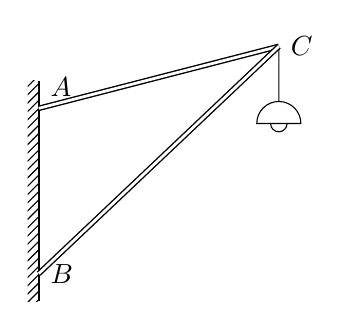
\begin{tikzpicture}[>=stealth,scale=0.7]
  \fill [pattern=north east lines](-2.2,-2) rectangle (-2,2);
  \draw[thick] (-2,2)--(-2,-2);
  \tkzDefPoints{-2/1.5/A,-2/-1.5/B,4/-1.5/b,2.5/1.5/a}
  \tkzInterCC(A,a)(B,b)\tkzGetPoints{C}{c}
  \tkzDefShiftPoint[C](0,-1){D}
  \draw (C)--(D);
  \draw (D) arc(90:0:0.4)--++(-0.8,0)arc(180:90:0.4);
  \draw ([yshift=-0.4cm,xshift=-0.15cm]D)arc(180:360:0.15);
  \pgfsetlinewidth{2pt}
  \pgfsetinnerlinewidth{1pt}
  \draw(A)node[above right]{$A$}--(C)node[right]{$C$};
  \draw(C)--(B)node[right]{$B$};
\end{tikzpicture}
\end{document}